\chapter{What Counts as a Law of Motion?}

Classical mechanics begins here with a question that is broader than any one orbit, any one falling stone, or any one charged particle. We want to know not only the specific laws governing particular systems, but also the general framework within which an acceptable law of motion must lie. Leonard Susskind therefore begins, quite deliberately, with absurdly simple worlds. The simplicity is not a detour. It is what allows the notions of state, law, determinism, conservation, and reversibility to emerge cleanly before the familiar machinery of mechanics is brought in. The present notes follow that unfolding closely, and the preserved board frames from LazyingArt LLC and Video2Book are used only where they steady a visible equation or diagram already motivated in the lecture.

\section{Two Questions and a Minimal World}

The lecture opens by separating two questions that are easy to mix together.

The first question is concrete: what are the laws for particular kinds of systems? A planet moving in the field of a heavy mass has one kind of law; a charged particle moving in a magnetic field has another. These are the specific laws of nature.

The second question is more structural: what counts as an allowable law at all? What must be true of a law of motion before we even begin to ask which particular system it describes? Susskind tells us immediately that this second question is the real target, while the first will merely supply illustrations.

So we begin with the smallest world that is still nontrivial. Let us take a coin lying on an abstract table. The only feature of the coin that matters is whether it is heads or tails. Thus the world contains one object with two configurations,
\[
H \qquad \text{and} \qquad T.
\]
An initial condition is just the choice of one of these configurations at the initial time. A law of motion is then a rule that tells us what happens next.

This order matters. First we decide what the possible configurations are. Only then do we ask how they evolve.

\section{A Coin as a Dynamical System}

For the coin, the configuration space is simply
\[
\mathcal{C}=\{H,T\}.
\]
Susskind first pauses over the vocabulary. This is our world. What is an initial condition? It is just the statement that the coin is heads or tails. What, then, is a law of motion? We are about to invent one.

He briefly remarks that there is an even simpler world: a one-sided coin. But that world is too simple, because nothing can happen in it. The two-state coin is the first place where the question becomes interesting.

Time is introduced in the simplest possible form. We imagine a stroboscopic world in which we look only at successive flashes, so the time variable is discrete:
\[
t\in\mathbb{Z}.
\]

\paragraph{The first law: nothing happens.}
The first law is as boring as possible:
\[
H\to H,\qquad T\to T.
\]
Heads remains heads, tails remains tails. This is a trivial law, but it is already a powerful one. Once the initial condition is known, the entire future is fixed. If the world begins in \(H\), its history is
\[
H,H,H,H,\dots
\]
and if it begins in \(T\), its history is
\[
T,T,T,T,\dots
\]

\paragraph{The second law: flip every step.}
There is only one other deterministic one-step law for a two-state system:
\[
H\to T,\qquad T\to H.
\]
At each flash of the stroboscope, the coin changes to the opposite state. Starting from heads, the history is
\[
H,T,H,T,\dots
\]
and starting from tails, it is
\[
T,H,T,H,\dots
\]

\begin{figure}
\centering

\includegraphics[width=0.78\textwidth]{lecture_01_figure_02.png}
\caption{The board layout for the two-state coin system: the boxed state set at left, the directed two-state cycle at center, and the explicit update rules beneath.}
\end{figure}

\begin{figure}
\centering
\begin{tikzpicture}[scale=1.0]
\draw (0,0) rectangle (2.2,1.3);
\node at (1.1,0.65) {$H,\ T$};

\draw (4.3,0.0) circle (0.45);
\draw (6.3,0.0) circle (0.45);
\node at (4.3,0.0) {$H$};
\node at (6.3,0.0) {$T$};

\draw[->] (4.62,0.28) .. controls (5.25,1.15) and (5.35,1.15) .. (5.98,0.28);
\draw[->] (5.98,-0.28) .. controls (5.35,-1.15) and (5.25,-1.15) .. (4.62,-0.28);

\node at (5.3,-1.75) {$H\to T,\qquad T\to H$};
\end{tikzpicture}
\caption{A clean reconstruction of the flip law.}
\end{figure}

Only after the pictures are in place does Susskind introduce notation. Let
\[
\sigma=
\begin{cases}
1,& \text{for } H,\\[4pt]
-1,& \text{for } T.
\end{cases}
\]
Then the two states are compressed into the two values of one variable. In that notation, the boring law becomes
\begin{equation}
\sigma(t+1)=\sigma(t),
\end{equation}
and the flip law becomes
\begin{equation}
\sigma(t+1)=-\sigma(t).
\end{equation}

\begin{figure}
\centering

\includegraphics[width=0.78\textwidth]{lecture_01_figure_03.png}
\caption{The same two-state system after the lecture upgrades it to sigma notation and writes the equation \(\sigma(t+1)=-\sigma(t)\).}
\end{figure}

\begin{figure}
\centering
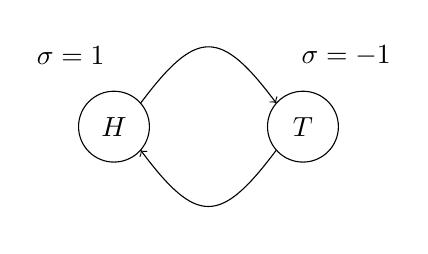
\begin{tikzpicture}[scale=1.0]
\draw (3.8,0.0) circle (0.45);
\draw (6.2,0.0) circle (0.45);
\node at (3.8,0.0) {$H$};
\node at (6.2,0.0) {$T$};
\node at (3.25,0.9) {$\sigma=1$};
\node at (6.75,0.9) {$\sigma=-1$};

\draw[->] (4.14,0.30) .. controls (4.85,1.25) and (5.15,1.25) .. (5.86,0.30);
\draw[->] (5.86,-0.30) .. controls (5.15,-1.25) and (4.85,-1.25) .. (4.14,-0.30);
\end{tikzpicture}
\caption{A clean reconstruction of the sigma-labeled state diagram.}
\end{figure}

This is the first important rhythm of the lecture: concept first, notation second. The symbol \(\sigma\) does not create the physics; it merely packages what was already clear from the update rule and the graph.

The coin itself is not the point. The point is that, for a closed system, a law of motion in classical mechanics is completely predictive. Once the law and the initial state are specified, the future is fixed.

\section{From a Coin to a Die: Cycles, Relabeling, and Conservation}

Now let us complicate the system, but not by much. Instead of a coin, take a die. The only fact about the die that matters for this discussion is that it has six possible states:
\[
1,2,3,4,5,6.
\]
An initial condition is again just a choice of one of these states.

At this stage Susskind does not try to write equations. The graph is the right language. A law of motion is a directed graph on the state space, and the history of the system is found by iterating the arrows.

The most boring law is again the one in which nothing happens: every state points to itself. More interesting is a single six-cycle,
\begin{equation}
1\to 2\to 3\to 4\to 5\to 6\to 1.
\end{equation}
One spoken line in the lecture is slightly garbled at this point, but the intended six-cycle is clear from the surrounding exposition and from the histories he derives from it.

\begin{figure}
\centering
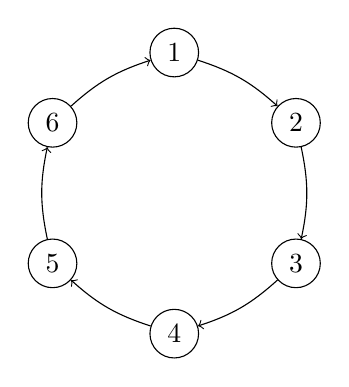
\begin{tikzpicture}[scale=1.05]
\node[circle,draw] (1) at (90:1.7) {$1$};
\node[circle,draw] (2) at (30:1.7) {$2$};
\node[circle,draw] (3) at (-30:1.7) {$3$};
\node[circle,draw] (4) at (-90:1.7) {$4$};
\node[circle,draw] (5) at (-150:1.7) {$5$};
\node[circle,draw] (6) at (150:1.7) {$6$};

\draw[->] (1) to[bend left=12] (2);
\draw[->] (2) to[bend left=12] (3);
\draw[->] (3) to[bend left=12] (4);
\draw[->] (4) to[bend left=12] (5);
\draw[->] (5) to[bend left=12] (6);
\draw[->] (6) to[bend left=12] (1);
\end{tikzpicture}
\caption{A law consisting of one six-cycle.}
\end{figure}

He then writes down a more awkward-looking law,
\[
1\to 2,\qquad 2\to 5,\qquad 5\to 3,\qquad 3\to 4,\qquad 4\to 6,\qquad 6\to 1,
\]
but this is not really a new kind of law. It is still one cycle passing through every state. The difference is only a relabeling. If we were to redraw the nodes in a different order, the graph would look just like the first one.

So what genuinely distinguishes different laws? Not the names we assign the states, but the cycle structure.

A genuinely new possibility is a graph with more than one disconnected cycle. For example,
\[
1\to 2\to 3\to 1,
\qquad
4\to 6\to 5\to 4.
\]
Now the die is still one system, but once the evolution begins, the state is trapped on one cycle or the other.

\begin{figure}
\centering
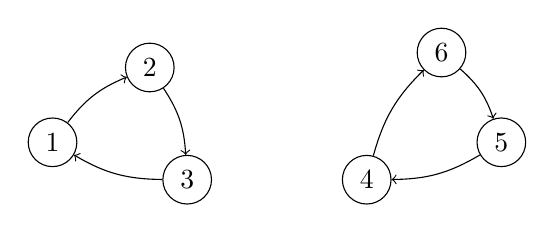
\begin{tikzpicture}[scale=0.95]
\node[circle,draw] (1) at (-3.0,1.0) {$1$};
\node[circle,draw] (2) at (-1.7,2.0) {$2$};
\node[circle,draw] (3) at (-1.2,0.5) {$3$};

\node[circle,draw] (4) at (1.2,0.5) {$4$};
\node[circle,draw] (5) at (3.0,1.0) {$5$};
\node[circle,draw] (6) at (2.2,2.2) {$6$};

\draw[->] (1) to[bend left=15] (2);
\draw[->] (2) to[bend left=15] (3);
\draw[->] (3) to[bend left=15] (1);

\draw[->] (4) to[bend left=15] (6);
\draw[->] (6) to[bend left=15] (5);
\draw[->] (5) to[bend left=15] (4);
\end{tikzpicture}
\caption{A law with two disconnected cycles.}
\end{figure}

This is where conservation first appears. We may assign one label to the upper cycle and another to the lower. That label remains fixed as the state moves around inside its cycle.

\begin{definition}
A conserved quantity is a label on the state space that remains constant under the evolution.
\end{definition}

In these finite examples, conserved quantities arise because the state space decomposes into disconnected pieces. Susskind then gives a further example with three cycles, including a fixed point, in order to emphasize that a conserved quantity need not specify the state completely. It may tell us only which orbit we belong to. The state changes; the conserved label does not.

\subsection{Question \& Answer}

\paragraph{Question.} What if the next step depends not only on the present configuration, but also on the previous one?

\paragraph{Answer.} Then the present configuration alone was never the full state. The state must be enlarged until the law again becomes one-step deterministic.

This is a crucial point, and Susskind does not let it pass too quickly. Suppose, for the coin, that what happens next depends on both the present face and the immediately preceding face. Then the correct state space is no longer \(\{H,T\}\). It is the four-element set
\[
\{HH,HT,TH,TT\},
\]
where, for example, \(HT\) means ``heads now, tails one step ago.''

So the right definition is not merely ``what the system looks like now.'' It is sharper:

\begin{definition}
The state of a system consists of all the information that must be specified at one time in order to predict the future.
\end{definition}

This principle will return in a much more serious form when we discuss particles. For the moment, the toy example has already done its work.

\section{Infinite State Spaces and the Meaning of an Allowed Law}

There is nothing in the discussion so far that requires the state space to be finite. We can just as well consider a particle that occupies one point on the infinite integer lattice,
\[
n\in\mathbb{Z}.
\]
The particle is still only one object. It simply has infinitely many possible states.

One possible law is
\begin{equation}
n(t+1)=n(t)+1.
\end{equation}
At each step the particle moves one unit to the right. If we think graphically, there is one endless orbit: going forward or backward, we pass through every integer.

A second law is
\begin{equation}
n(t+1)=n(t)+2.
\end{equation}
Now the odd integers communicate only with odd integers, and the even integers only with even integers. So parity is conserved.

\begin{figure}
\centering
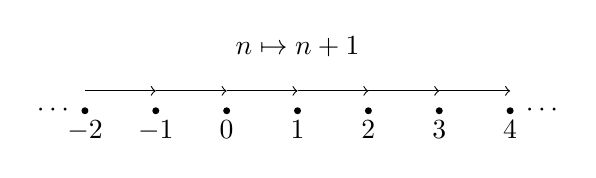
\begin{tikzpicture}[scale=0.9]
\foreach \x/\lab in {0/{-2},1/{-1},2/{0},3/{1},4/{2},5/{3},6/{4}}{
  \fill (\x,0) circle (1.4pt);
  \node[below] at (\x,0) {$\lab$};
}
\foreach \x in {0,1,2,3,4,5}{
  \draw[->] (\x,0.28) -- (\x+1,0.28);
}
\node at (3,0.9) {$n\mapsto n+1$};
\node at (-0.45,0) {$\cdots$};
\node at (6.45,0) {$\cdots$};
\end{tikzpicture}

\vspace{0.8cm}

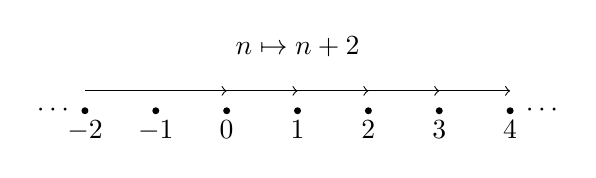
\begin{tikzpicture}[scale=0.9]
\foreach \x/\lab in {0/{-2},1/{-1},2/{0},3/{1},4/{2},5/{3},6/{4}}{
  \fill (\x,0) circle (1.4pt);
  \node[below] at (\x,0) {$\lab$};
}
\foreach \x in {0,1,2,3,4}{
  \draw[->] (\x,0.28) -- (\x+2,0.28);
}
\node at (3,0.9) {$n\mapsto n+2$};
\node at (-0.45,0) {$\cdots$};
\node at (6.45,0) {$\cdots$};
\end{tikzpicture}
\caption{Two infinite-state laws on the integer lattice. The second preserves parity.}
\end{figure}

A convenient encoding is
\[
Q_{\mathrm{parity}}(n)=
\begin{cases}
0,& n \text{ even},\\[4pt]
1,& n \text{ odd}.
\end{cases}
\]
Under \(n\mapsto n+2\), this quantity is unchanged. Thus the language of cycles, conserved quantities, and deterministic evolution survives the move from finite to infinite state spaces.

But now the lecture reaches its sharpest conceptual pivot. The laws we have written so far have all shared an additional feature: not only do they predict the future, they also determine the past. Susskind now draws a law that is deterministic forward but not backward.

Take a three-state system with states \(H\), \(T\), and \(E\) (for ``edge''). Let the arrows be
\[
H\to T,\qquad T\to E,\qquad E\to T.
\]
This law predicts the future perfectly. If we start at \(H\), we get
\[
H,T,E,T,E,\dots
\]
and if we start at \(T\), we get
\[
T,E,T,E,\dots
\]
But if all we know is that the present state is \(T\), we do not know where we came from. The previous state could have been \(H\) or \(E\).

\begin{figure}
\centering
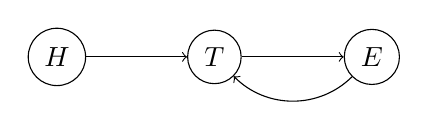
\begin{tikzpicture}[scale=1.0]
\node[circle,draw] (H) at (-2,0) {$H$};
\node[circle,draw] (T) at (0,0) {$T$};
\node[circle,draw] (E) at (2,0) {$E$};

\draw[->] (H) -- (T);
\draw[->] (T) -- (E);
\draw[->] (E) to[bend left=45] (T);
\end{tikzpicture}
\caption{A future-deterministic law that is not reversible.}
\end{figure}

\subsection{Question \& Answer}

\paragraph{Question.} Why is this law disallowed, if it still predicts the future?

\paragraph{Answer.} Because classical mechanics demands more than forward predictability. It demands reversibility.

Susskind's test is beautifully simple: reverse every arrow. In the reversed graph, if we stand at \(T\), we do not know which way to go next. There are two possibilities. So the reversed evolution is not predictive. The original law runs forward but cannot be run backward uniquely.

\begin{definition}
A law is reversible if the present state determines both the next state and the previous state. In the graph language, each state must have exactly one outgoing arrow and exactly one incoming arrow.
\end{definition}

This is the real payoff of the first half of the lecture. A legal classical law is not merely deterministic into the future. It is deterministic into the past as well.

Susskind briefly remarks that probabilistic laws also fall outside the classical framework as he is defining it here. That larger comparison is postponed. For the present lecture, the essential distinction is already on the board: future determinism is not enough.

\section{Exact Laws, Imperfect Initial Data, and the Pivot to Particles}

At this point we might be tempted to say: classical mechanics predicts everything. Susskind immediately softens that slogan.

To predict the future we need two ingredients:
\begin{itemize}
\item the law of motion,
\item the initial condition.
\end{itemize}
A perfectly exact law is of no practical use if the initial condition is only imperfectly known.

In the toy systems this problem seems mild. One can imagine simply looking at the coin and reading its initial state exactly. But the real world is different. The degrees of freedom are continuous. Positions and velocities are real numbers, and no matter how many decimal places we measure, we never know them perfectly.

Thus there is a gap between exact determinism and practical predictability. Some systems magnify tiny initial errors. The weather is Susskind's example. If the atmospheric state is known only approximately, then after a long enough time the uncertainty blows up, and prediction fails in practice even though the underlying equations remain exact.

So the right classical statement is more careful. If we knew the initial conditions perfectly, then a true classical system would determine both future and past forever. If we know them only approximately, then we must ask how long that approximation remains useful.

This qualification does not undo determinism. It places it where it belongs: in the law itself, not in our practical ability to exploit it.

Only after making that distinction does Susskind turn to the more realistic world of particles. We are now ready to ask what the configurations of a point particle are. But before we do so, he stops and says exactly what the lecture needs next: a little mathematical preliminary.

\section{Coordinates, Vectors, and the Algebra We Need}

A coordinate system is simply a quantitative way to describe space. For the moment we take space to be three-dimensional, so a point is described by three coordinates,
\[
(x,y,z),
\qquad \text{or equivalently} \qquad
(x_1,x_2,x_3).
\]
We choose an origin, three mutually perpendicular axes, an orientation, and a system of units. Once the \(x\)- and \(y\)-axes are fixed, there remains one discrete choice for the direction of the \(z\)-axis, and the lecture adopts the standard right-handed convention.

\begin{figure}
\centering
\begin{tikzpicture}[scale=1.15]
\draw[->] (0,0) -- (2.5,0) node[right] {$x$};
\draw[->] (0,0) -- (0,2.4) node[above] {$y$};
\draw[->] (0,0) -- (-1.3,-0.9) node[below] {$z$};

\fill (1.6,1.35) circle (1.2pt);
\draw[->] (0,0) -- (1.6,1.35) node[midway, above left] {$\vec r$};
\draw[dashed] (1.6,1.35) -- (1.6,0);
\draw[dashed] (1.6,1.35) -- (0,1.35);
\node[below] at (1.6,0) {$x$};
\node[left] at (0,1.35) {$y$};
\end{tikzpicture}
\caption{A point in a right-handed Cartesian coordinate system, together with its position vector.}
\end{figure}

Now let us recall what a vector is. A vector is an object with magnitude and direction. The first example is the position of a point relative to the origin, but Susskind is careful to say that the notion of vector is more general than that. It may represent position, velocity, acceleration, an electric field, or any other quantity with length and direction.

Equally important is what a vector is not. It is not, in the first instance, tied to a particular place in space. If we slide the arrow without changing its length or direction, we have the same vector.

If a vector has components \((v_x,v_y,v_z)\), then its magnitude is
\begin{equation}
|\vec v|=\sqrt{v_x^2+v_y^2+v_z^2}.
\end{equation}
The direction is encoded in the ratios of the components.

We can multiply a vector by an ordinary real number. If \(c>0\), the vector \(c\vec A\) has the same direction as \(\vec A\) and magnitude \(c|\vec A|\). If \(c<0\), the direction is reversed. In particular, \(-\vec A\) points opposite to \(\vec A\).

We can also add vectors. The lecture presents three equivalent pictures:
\begin{itemize}
\item place the tail of \(\vec B\) at the head of \(\vec A\), and the third side of the triangle is \(\vec A+\vec B\);
\item place the tails of \(\vec A\) and \(\vec B\) together, complete the parallelogram, and take the diagonal;
\item add components:
\[
C_i=A_i+B_i.
\]
\end{itemize}
This last form is often the most useful in calculation.

Susskind then asks the natural next question. If vectors can be added, subtracted, and multiplied by numbers, can they be multiplied with each other? The answer is yes, but not in the ordinary scalar sense. The simplest such product is the dot product.

Geometrically, \(\vec A\cdot\vec B\) is obtained by taking the component of \(\vec A\) along the axis defined by \(\vec B\), and multiplying by the magnitude of \(\vec B\). If \(\theta\) is the angle between them, this gives
\begin{equation}
\vec A\cdot \vec B = |\vec A|\,|\vec B|\cos\theta.
\end{equation}
Because this formula is symmetric in \(\vec A\) and \(\vec B\), it makes manifest that
\[
\vec A\cdot\vec B=\vec B\cdot\vec A.
\]

In components, the same quantity is
\begin{equation}
\vec A\cdot\vec B=A_xB_x+A_yB_y+A_zB_z.
\end{equation}
In particular,
\begin{equation}
\vec A\cdot\vec A=|\vec A|^2.
\end{equation}
This is precisely what makes the dot product useful. It lets us compute angles and test perpendicularity directly from components. If the dot product vanishes, the vectors are perpendicular. If it is negative, the angle between them is greater than \(90^\circ\).

\begin{figure}
\centering

\includegraphics[width=0.70\textwidth]{lecture_01_figure_04.png}
\caption{The lecture board at the vector-subtraction step leading to the law of cosines.}
\end{figure}

The law of cosines is then derived from the dot product. Here the live rhythm of the lecture matters: Susskind first says \(\vec C=\vec A+\vec B\), then stops, corrects himself, and says that for the side drawn in the sketch we need
\[
\vec C=\vec A-\vec B.
\]
That correction should be preserved, because it shows the argument unfolding rather than arriving fully polished from nowhere.

Now we compute:
\begin{align}
|\vec C|^2
  &= \vec C\cdot\vec C \\
  &= (\vec A-\vec B)\cdot(\vec A-\vec B) \\
  &= \vec A\cdot\vec A+\vec B\cdot\vec B-2\vec A\cdot\vec B \\
  &= |\vec A|^2+|\vec B|^2-2|\vec A|\,|\vec B|\cos\theta.
\end{align}
This is the law of cosines. The transcript momentarily garbles the last phrase as ``cosine of the length,'' but the mathematics is unambiguous: it is the cosine of the angle.

\begin{figure}
\centering
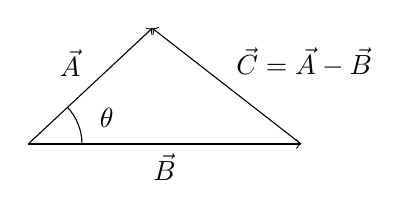
\begin{tikzpicture}[scale=1.05]
\coordinate (O) at (0,0);
\coordinate (A) at (1.5,1.4);
\coordinate (B) at (3.3,0);

\draw[->] (O) -- (A) node[midway, above left] {$\vec A$};
\draw[->] (O) -- (B) node[midway, below] {$\vec B$};
\draw[->] (B) -- (A) node[midway, above right] {$\vec C=\vec A-\vec B$};

\draw (0.65,0) arc (0:43:0.65);
\node at (0.95,0.32) {$\theta$};
\end{tikzpicture}
\caption{A clean reconstruction of the vector-subtraction triangle used in the derivation.}
\end{figure}

By this point the lecture has done its mathematical preparation. We have coordinates, vectors, component notation, vector addition, scalar multiplication, and the dot product. Now we can use them.

\section{Position, Velocity, Acceleration, and Two Motion Examples}

The position of a particle relative to the chosen origin defines a distinguished vector,
\[
\vec r(t).
\]
Its components are just the coordinates of the particle:
\[
\vec r(t)=(x(t),y(t),z(t)).
\]
The notation \(r\) is traditional; Susskind remarks that it presumably comes from ``radius,'' though here it simply means position vector.

Because classical mechanics concerns motion, \(\vec r\) is in general a function of time. Thus the motion of a particle in three-dimensional space is encoded by the three functions
\[
x(t),\qquad y(t),\qquad z(t).
\]

The next concept is velocity. It is also a vector, and it need not point in the same direction as \(\vec r\). Its definition is
\begin{equation}
v_i=\frac{dx_i}{dt}=\dot x_i,
\end{equation}
or, in vector form,
\begin{equation}
\vec v=\frac{d\vec r}{dt}=\dot{\vec r}.
\end{equation}
The dot notation is introduced at this point as a special shorthand for differentiation with respect to time only.

Acceleration is the rate of change of velocity. It too is a vector:
\begin{equation}
a_i=\frac{dv_i}{dt}=\dot v_i=\ddot x_i,
\qquad
\vec a=\frac{d\vec v}{dt}=\frac{d^2\vec r}{dt^2}=\ddot{\vec r}.
\end{equation}

\begin{figure}
\centering

\includegraphics[width=0.78\textwidth]{lecture_01_figure_05.png}
\caption{The lecture board moving from component notation to the compact vector statement \(\vec v=d\vec r/dt\).}
\end{figure}

The screenshot shows uppercase \(V_i\) and \(X_i\) on the board. The surrounding lecture, however, does not insist on that convention, and for consistency we normalize to lower-case component notation in the text.

Now that the concepts are in hand, the lecture does exactly what it promised: let us work out an example or two.

\paragraph{First example: motion along a line.}
If the particle moves only along the \(x\)-axis, then it is hardly worth speaking of vectors at all. We may simply write
\begin{equation}
x(t)=a+bt+ct^2.
\end{equation}
At \(t=0\), the particle is at \(x=a\). Differentiating once gives the velocity,
\begin{equation}
\dot x(t)=b+2ct,
\end{equation}
and differentiating again gives the acceleration,
\begin{equation}
\ddot x(t)=2c.
\end{equation}
So the acceleration is constant. This is uniformly accelerated motion, the prototype of motion in a constant gravitational field.

\paragraph{Second example: uniform circular motion.}
The final example is more revealing. Consider a particle moving on the unit circle in the \(xy\)-plane. We ignore the \(z\)-direction. Let the angle grow linearly with time:
\begin{equation}
\theta(t)=\omega t.
\end{equation}
One full revolution corresponds to \(\theta=2\pi\), so the period is
\begin{equation}
T=\frac{2\pi}{\omega}.
\end{equation}
The transcript momentarily stumbles at the period formula, but the final expression is clear and standard.

On the unit circle, the position components are
\begin{equation}
x(t)=\cos(\omega t),\qquad y(t)=\sin(\omega t).
\end{equation}

\begin{figure}
\centering
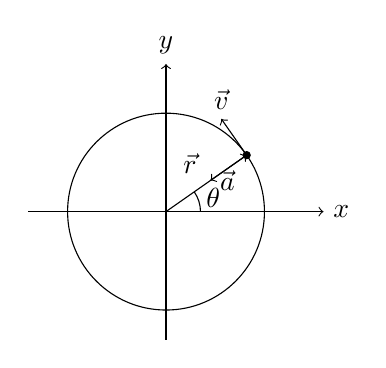
\begin{tikzpicture}[scale=1.25]
\draw[->] (-1.4,0) -- (1.6,0) node[right] {$x$};
\draw[->] (0,-1.3) -- (0,1.5) node[above] {$y$};
\draw (0,0) circle (1);

\coordinate (P) at ({cos(35)},{sin(35)});
\fill (P) circle (1.2pt);

\draw[->] (0,0) -- (P) node[midway, above left] {$\vec r$};
\draw[->] (P) -- ++({-0.45*sin(35)},{0.45*cos(35)}) node[above] {$\vec v$};
\draw[->] (P) -- ++({-0.45*cos(35)},{-0.45*sin(35)}) node[right] {$\vec a$};

\draw (0.35,0) arc (0:35:0.35);
\node at (0.48,0.14) {$\theta$};
\end{tikzpicture}
\caption{Uniform circular motion on the unit circle. The velocity is tangent to the orbit, while the acceleration points inward.}
\end{figure}

Differentiating once, we find the velocity components:
\begin{equation}
v_x(t)=-\omega\sin(\omega t),\qquad v_y(t)=\omega\cos(\omega t).
\end{equation}

\subsection{Question \& Answer}

\paragraph{Question.} It looks obvious that the velocity is perpendicular to the position vector. How do we prove it?

\paragraph{Answer.} We prove it with the dot product:
\begin{align}
\vec r\cdot\vec v
  &= x v_x + y v_y \\
  &= \cos(\omega t)\bigl(-\omega\sin(\omega t)\bigr)
   + \sin(\omega t)\bigl(\omega\cos(\omega t)\bigr) \\
  &= 0.
\end{align}
Since the dot product vanishes, \(\vec r\) and \(\vec v\) are perpendicular.

This is one of the lecture's nicest little moments. First we trust the geometry. Then we check it algebraically. The calculation does not replace the picture; it confirms it.

Differentiating once more, we obtain the acceleration:
\begin{equation}
a_x(t)=-\omega^2\cos(\omega t),\qquad a_y(t)=-\omega^2\sin(\omega t).
\end{equation}
Therefore
\begin{equation}
\vec a=-\omega^2\vec r.
\end{equation}
So the acceleration is parallel to \(\vec r\) but points in the opposite direction. It is inward, toward the origin. The spoken phrase ``centrifugal acceleration'' in the lecture is evidently a slip; the mathematics is perfectly clear.

Finally, the magnitudes are
\begin{align}
|\vec v|^2
  &= v_x^2+v_y^2 \\
  &= \omega^2\sin^2(\omega t)+\omega^2\cos^2(\omega t) \\
  &= \omega^2,
\end{align}
hence
\[
|\vec v|=\omega.
\]
Likewise,
\begin{align}
|\vec a|^2
  &= a_x^2+a_y^2 \\
  &= \omega^4\cos^2(\omega t)+\omega^4\sin^2(\omega t) \\
  &= \omega^4,
\end{align}
so
\[
|\vec a|=\omega^2.
\]

The closing example is not an afterthought. It is where the formalism becomes mechanics again: position, velocity, acceleration, orthogonality, inward acceleration, and the concrete role of \(\omega\).

\section{Summary}

The lecture begins by asking what an allowable law of motion must look like, and it answers that question before ever discussing a planet or a force. Coins, dice, and integer lattices are enough to reveal the structure: a state space, an initial condition, an update rule, deterministic evolution, conserved quantities, and, crucially, reversibility.

Only after that conceptual warm-up does the lecture move to particles in space. There we build the coordinate and vector language that mechanics will need: components, magnitudes, vector addition, the dot product, and the law of cosines. With those tools in hand, position, velocity, and acceleration follow naturally, and the two final examples show the formalism at work. The next step, exactly as Susskind says at the end of the lecture, is to return to particles and ask the full dynamical question: what is the space of initial conditions, and what laws move a particle from one instant to the next?